\begin{frame}{Back to theory: from erasures to errors}
\end{frame}
%-----------------------------------------------------------------------
\begin{frame}\frametitle{Finite field with $p$ elements}
\begin{block}{$p$ is prime}
\begin{itemize}
\item $\mathbb{F}_p - \{0,1,2,\ldots,p-1\}$
\item $a \oplus b = (a+b) \mod p$
\item $a \odot b = (ab) \mod p$
\item We can $+,\times,\div$, inverses
\item $W$ is a (primitive) element such that $1,W,W^2,\ldots,W^{p-1}$ are distinct
\end{itemize}
\end{block}
\pause
\begin{block}{Example $\mathbb{F}_5$}
\begin{itemize}
\item $W=2$
\item $W^0=1, W^1=2, W^2 = 4, W^3 = 3$
\end{itemize}
\end{block}
\pause
\begin{block}{$p$ need not be prime}
\begin{itemize}
\item Everything can be extended to finite fields with $q = 2^r$ elements
\item May be extended to integers - not sure
\end{itemize}
\end{block}
\end{frame}
%-------------------------------------------------------------
\begin{frame}{$p$-symmetric channel and error correction}

\begin{figure}[t]
\centering
\scalebox{0.55}{%\documentclass{article}
%
%\usepackage{tikz}
%\usetikzlibrary{arrows,shapes,chains,matrix,positioning,scopes,patterns,calc}
%\usepackage{color}
%
%\usepackage{latexsym}
%\usepackage{amsmath,amssymb,amsthm}
%\usepackage{etoolbox}
%
%\begin{document}

\begin{tikzpicture}
\def \recW{1in}; %Encoder Length
\def \recH{0.5in}; %Encoder Width

\def \R{0.06in}; %Larger circle radius

\def \Gblks{0.25in}; %Gaps between blocks
\def \ext{0.95in}; %Extensions towards left and right of the figure
\def \extB{0.25in}; %Extensions towards top of the figure

\def \fsizes{\normalsize}; %Defining a generic font size to be adjusted depending on the scaling
\def \fsize{\Large}; %Defining a generic font size to be adjusted depending on the scaling

\tikzstyle{rect}   = [ rectangle, draw, text centered, thick,
                        minimum height=\recH, minimum width=\recW ]

\node [rect](enc) at (0,0) {\fsizes{Encoder}} ;
\node (chan)  [right = \ext of enc,draw,rectangle,text centered,thick,minimum width=1.5in,minimum height=1.5in]    {\includegraphics[width=1.5in,height=1.5in,angle=-90]{Parysymmetricchannelmodel.pdf}};
\node (dec)[rect,right=\ext of chan] {\fsizes Decoder} ;

\draw[<-,thick](enc)-- +(-2*\ext,0) node[midway,above]{\fsize $m_1,\ldots,m_k$};
\draw[->,thick](enc)--(chan)node[midway,above]{\fsize $x_1,\ldots,x_n$}node[midway,below]{\fsize $x_i\in \mathbb{F}_p$};
\draw[->,thick](chan)--(dec)node[midway,above]{\fsize $r_1,\ldots,r_n$}node[midway,below]{\fsize $r_i\in \mathbb{F}_p$};;

%\draw[<-,thick](chan)--+(0,\extB) node[above] {\fsize $e_1,\ldots,e_n$};
\draw[->,thick](dec)--+(2*\ext,0)node[midway,above]{\fsize  $\hat{m_1},\ldots,\hat{m_k}$};

\end{tikzpicture}
%\end{document} }
\end{figure}

\begin{block}{Error correction coding}
\begin{itemize}
%\item Capacity $C = 1-H_2(\epsilon)$
\item Another simple channel model which has been extensively considered
\item Has been the canonical model for algebraic coding theorists
\end{itemize}
\end{block}
%\vspace*{-5mm}
%\begin{figure}[t]
%\centering
%\includegraphics[width=1.5in,angle=-90]{./Figures/Parysymmetricchannelmodel}
%\end{figure}
\end{frame}

%--------------------------------------------------------------------------------------
\begin{frame}{Generalized LDPC code and error channels}
\vspace{-7mm}
\begin{figure}[t]
\centering
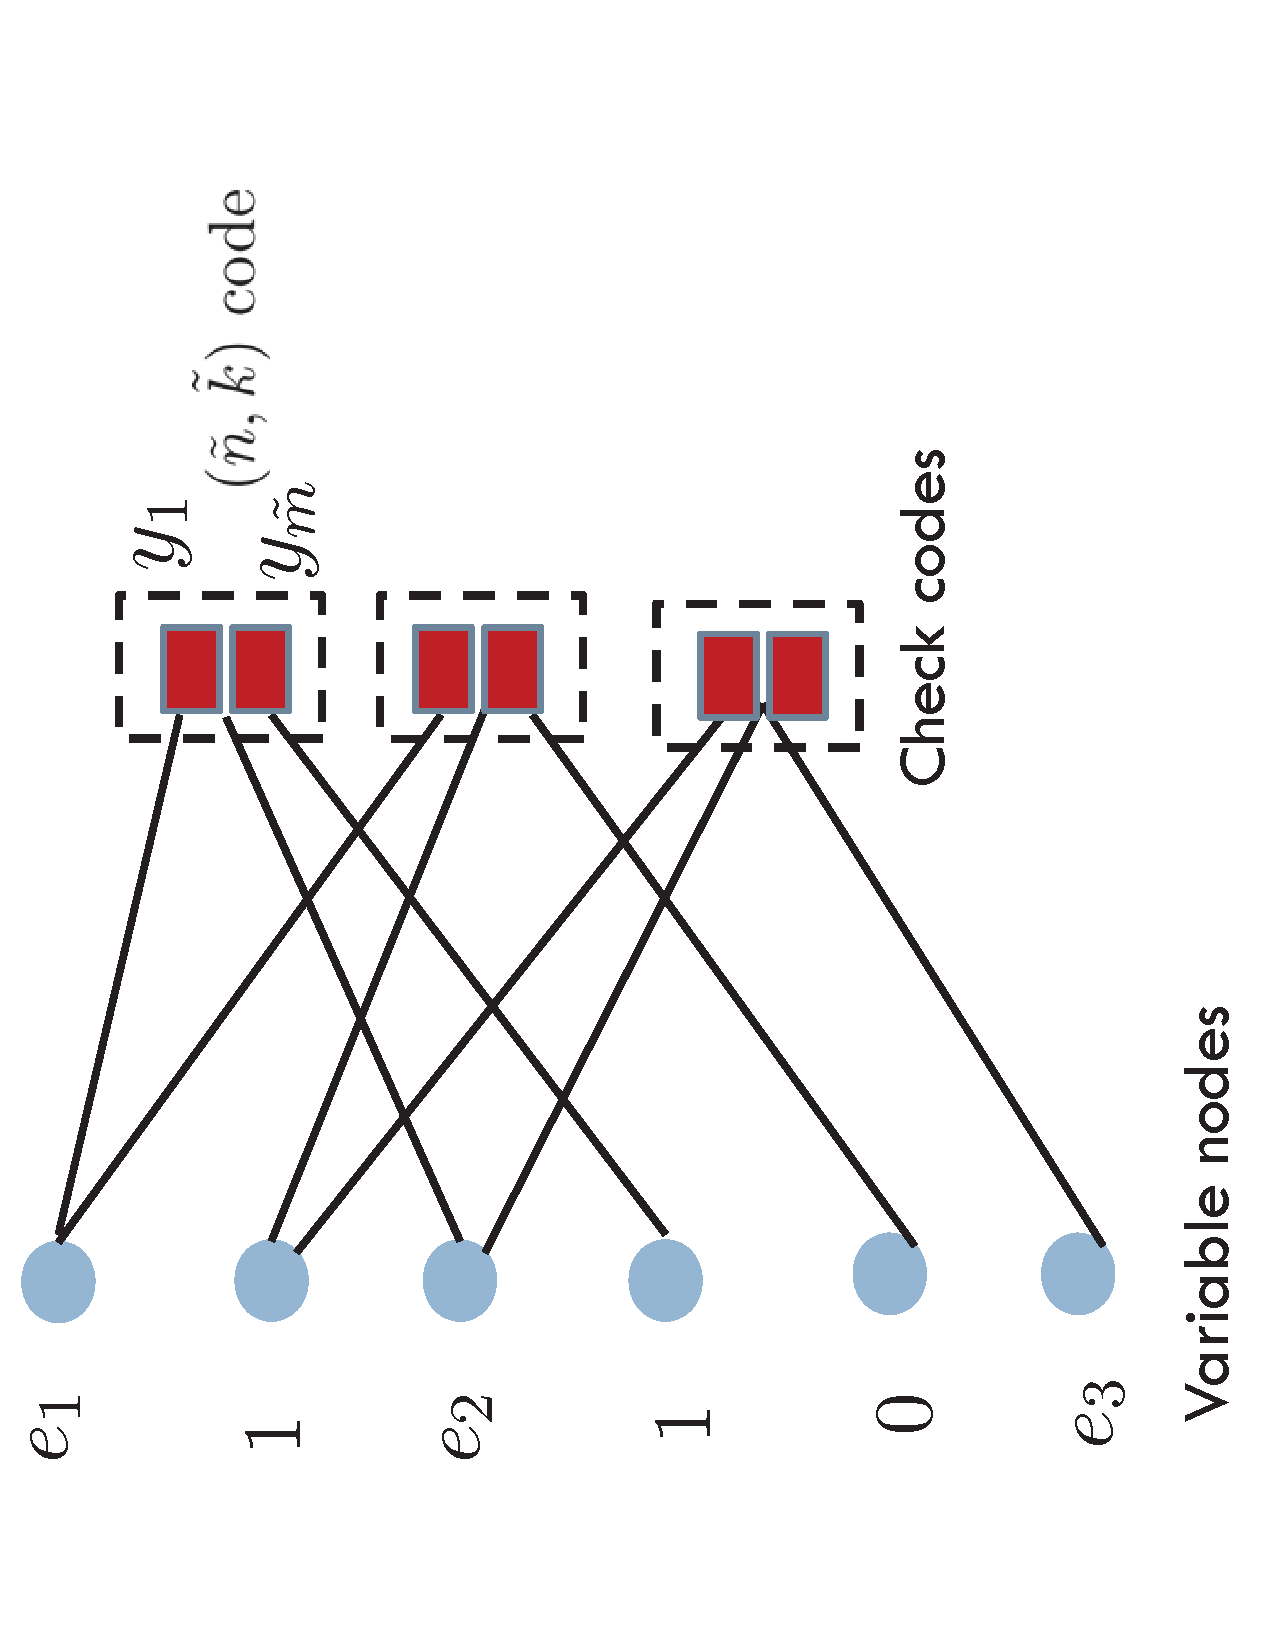
\includegraphics[width=2.15in,angle=-90]{./Figures/GLDPC}
\end{figure}

\begin{block}{}
\begin{itemize}
\item GLDPC introduced by Tanner in 1981
\item Each check is a $(\tilde{n},\tilde{k})$, $t$-error correcting code
\item If there are $\leq t$ errors in a check, it can be recovered
%\item Density evolution equations can be written and thresholds computed
\item For now, assume no miscorrections
\end{itemize}
\end{block}
\end{frame}
%--------------------------------------------------------------------------------------
\begin{frame}{Peeling process is same for erasure and error channels}
\begin{columns}
\column{0.5\textwidth}
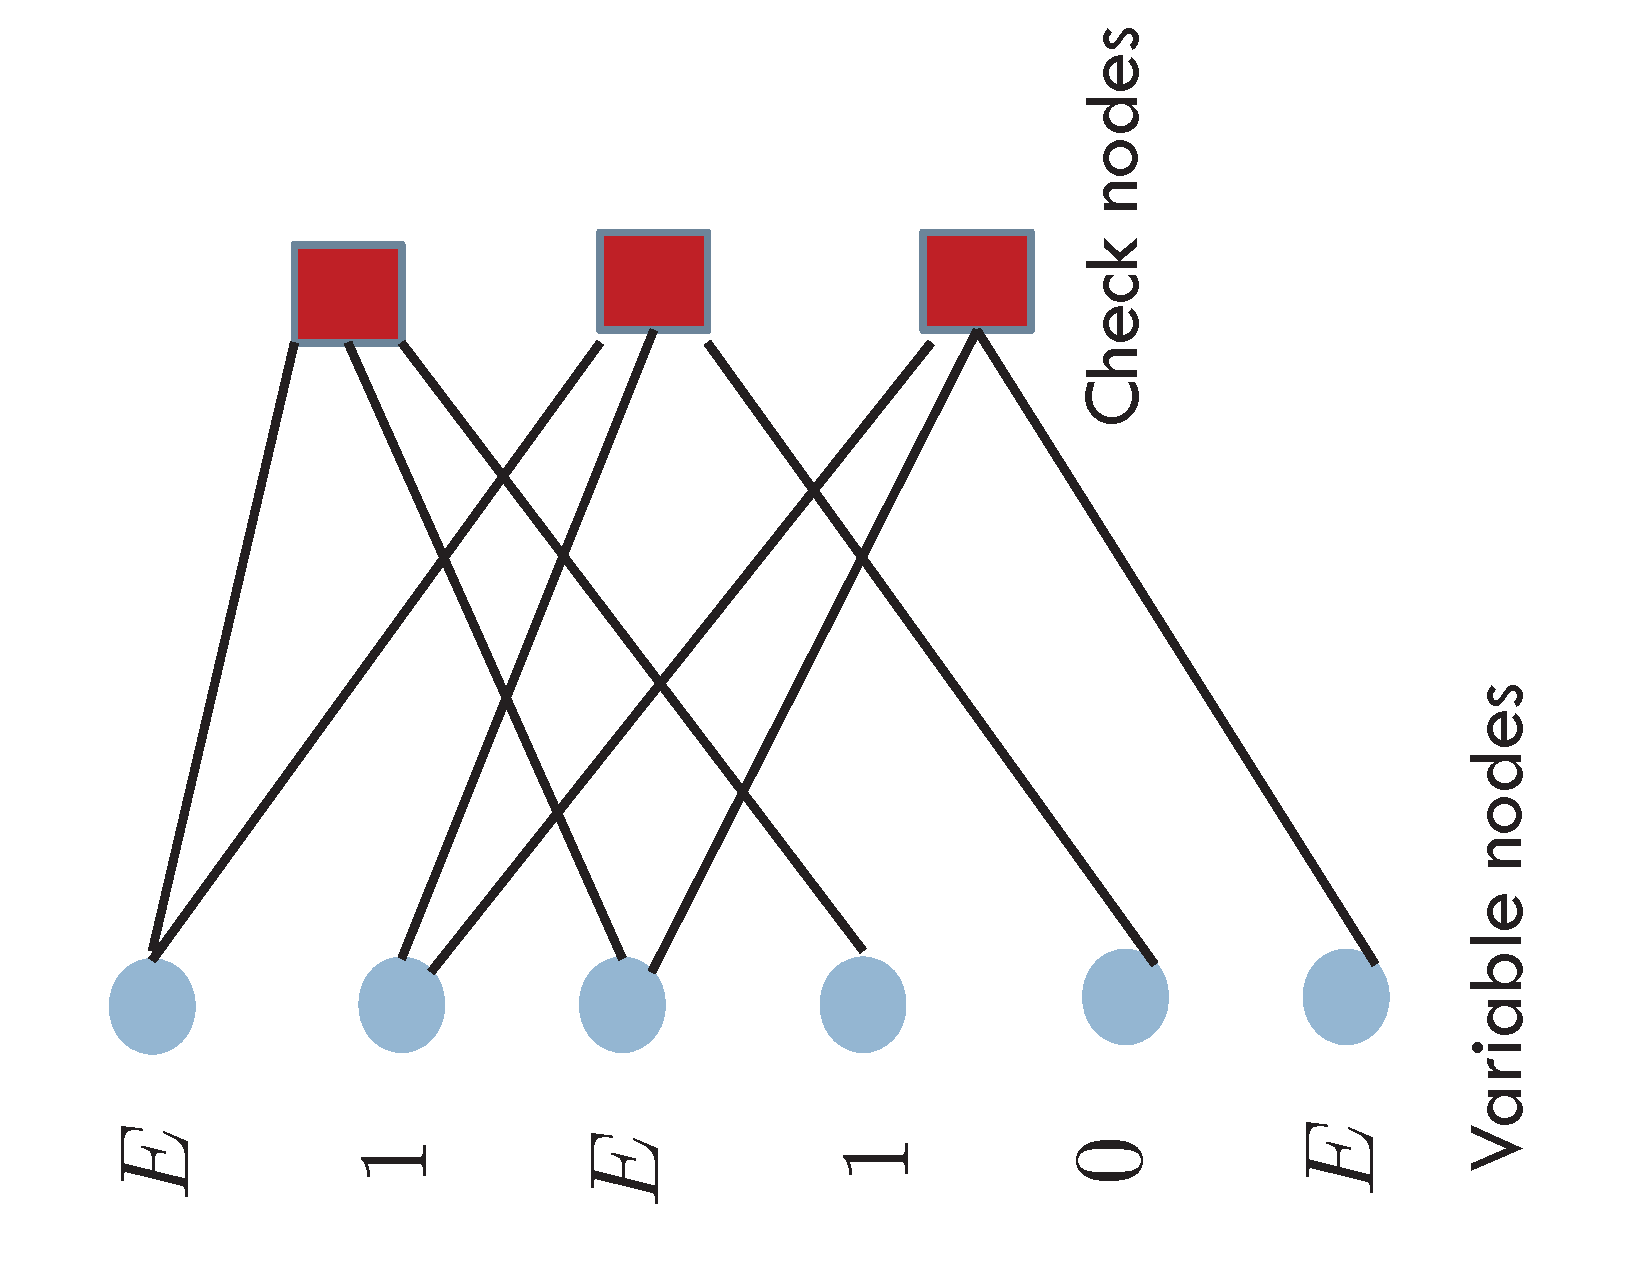
\includegraphics[width=2.3in,angle=-90]{./Figures/Tannergraph63codewitherasures}
\column{0.5\textwidth}
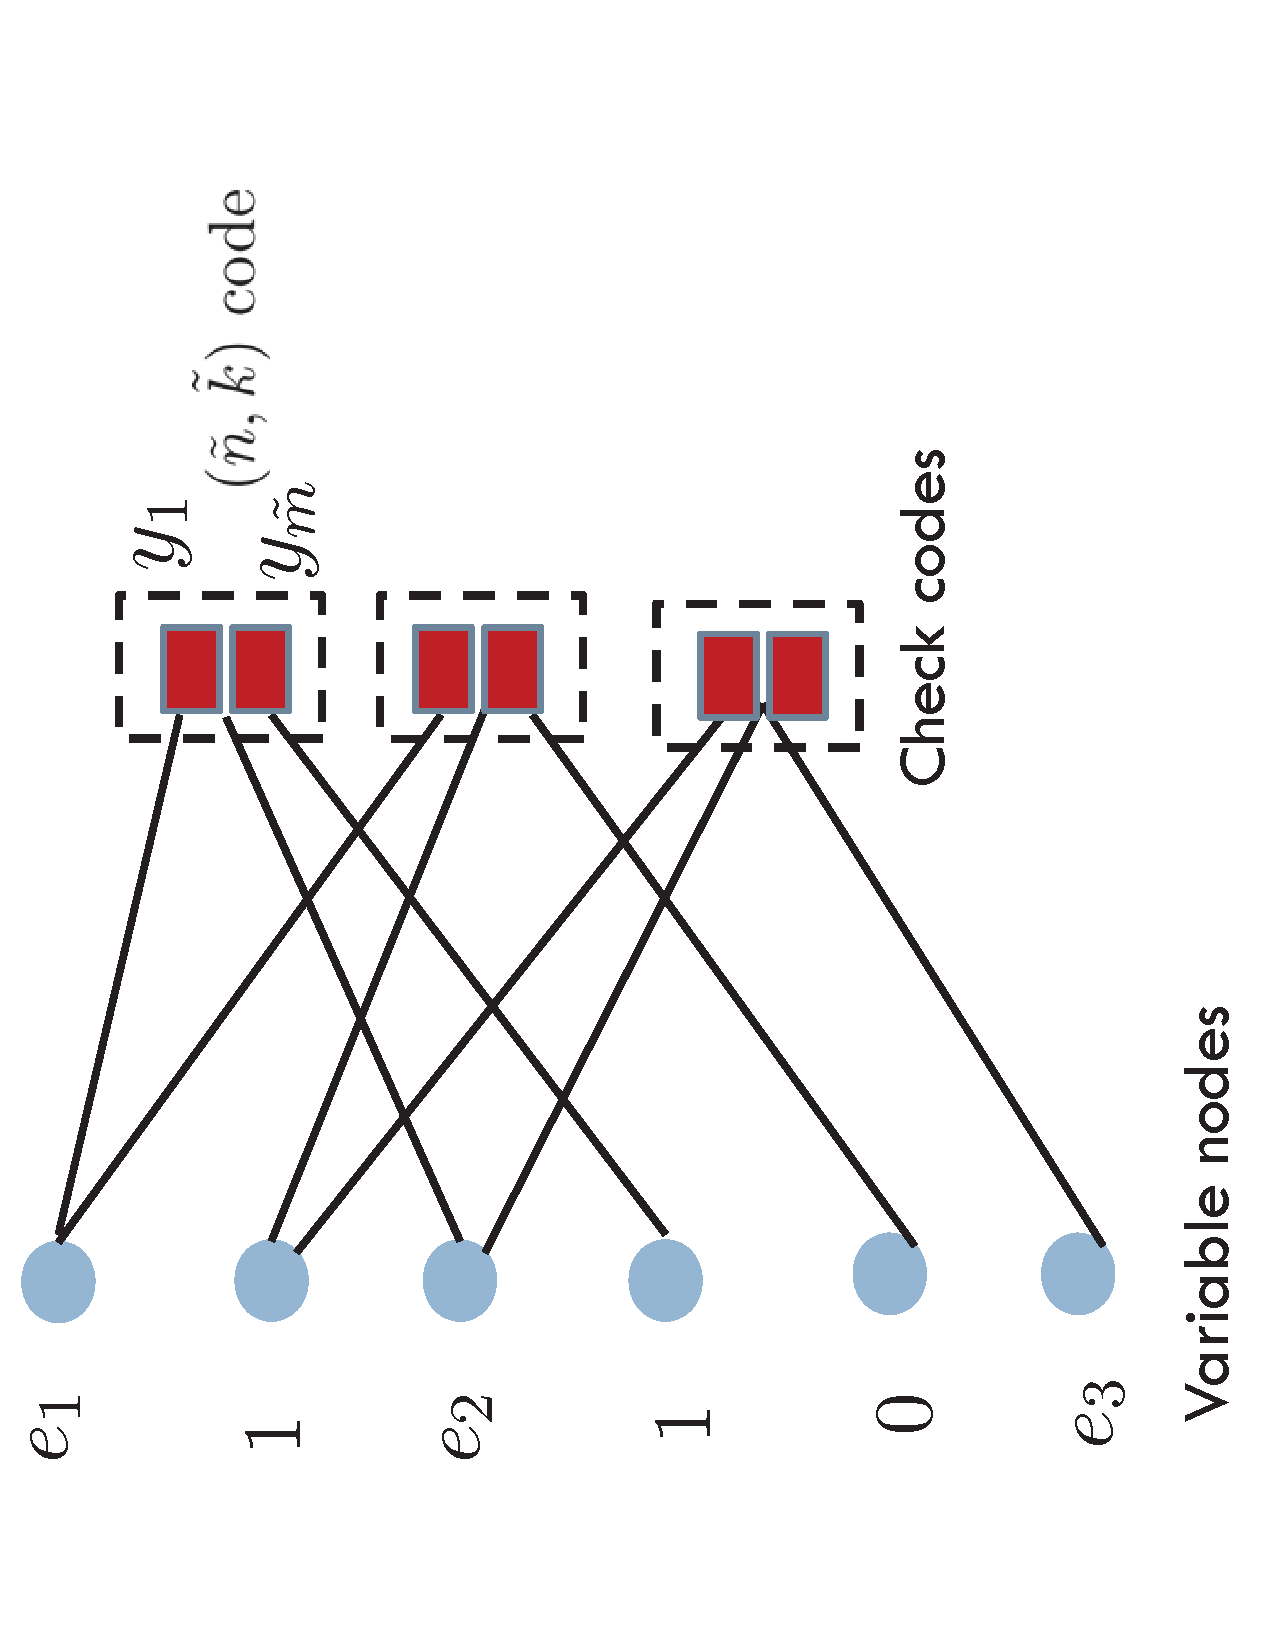
\includegraphics[width=2.15in,angle=-90]{./Figures/GLDPC}
\end{columns}
\begin{block}{}
\begin{itemize}
  \item Assume 1-error correcting check code and no miscorrections
  \item One-to-one correspondence between messages passed - DE can be used
  \item Not optimal for the error channel but it is not bad at high rates
  \item Spatially coupled versions are optimal at high rates (Jian, Pfister and N)
\end{itemize}
\end{block}
\end{frame}
%--------------------------------------------------------------------------------------
\begin{frame}\frametitle{Erasures to errors - tensoring and peeling}
\begin{columns}
    \column{.45\textwidth}
    \small
    \[
    H = \left[
    \begin{array}{ccccccc}
    1&0&1&1&0&0\\
    1&1&0&0&1&0 \\
    0&1&1&0&0&1
    \end{array}
    \right]
    \]
    \[
    \otimes
    \]
    \[
    B = \left[
    \begin{array}{ccccccc}
    1&1&1&1&1&1\\
    1&W&W^2&W^3&W^4&W^5
    \end{array}
    \right]
    \]
    \[
    \mathbf{\tilde{H}} = \left[
    \begin{array}{ccccccc}
    1&0&1&1&0&0\\
    1&0&W^2&W^3&0&0\\
    1&1&0&0&1&0 \\
    1&W&0&0&W^4&0 \\
    0&1&1&0&0&1 \\
    0&W&W^2&0&0&W^5
    \end{array}
    \right]
    \]
    \column{.45\textwidth}
    \begin{figure}[t]
    \centering
    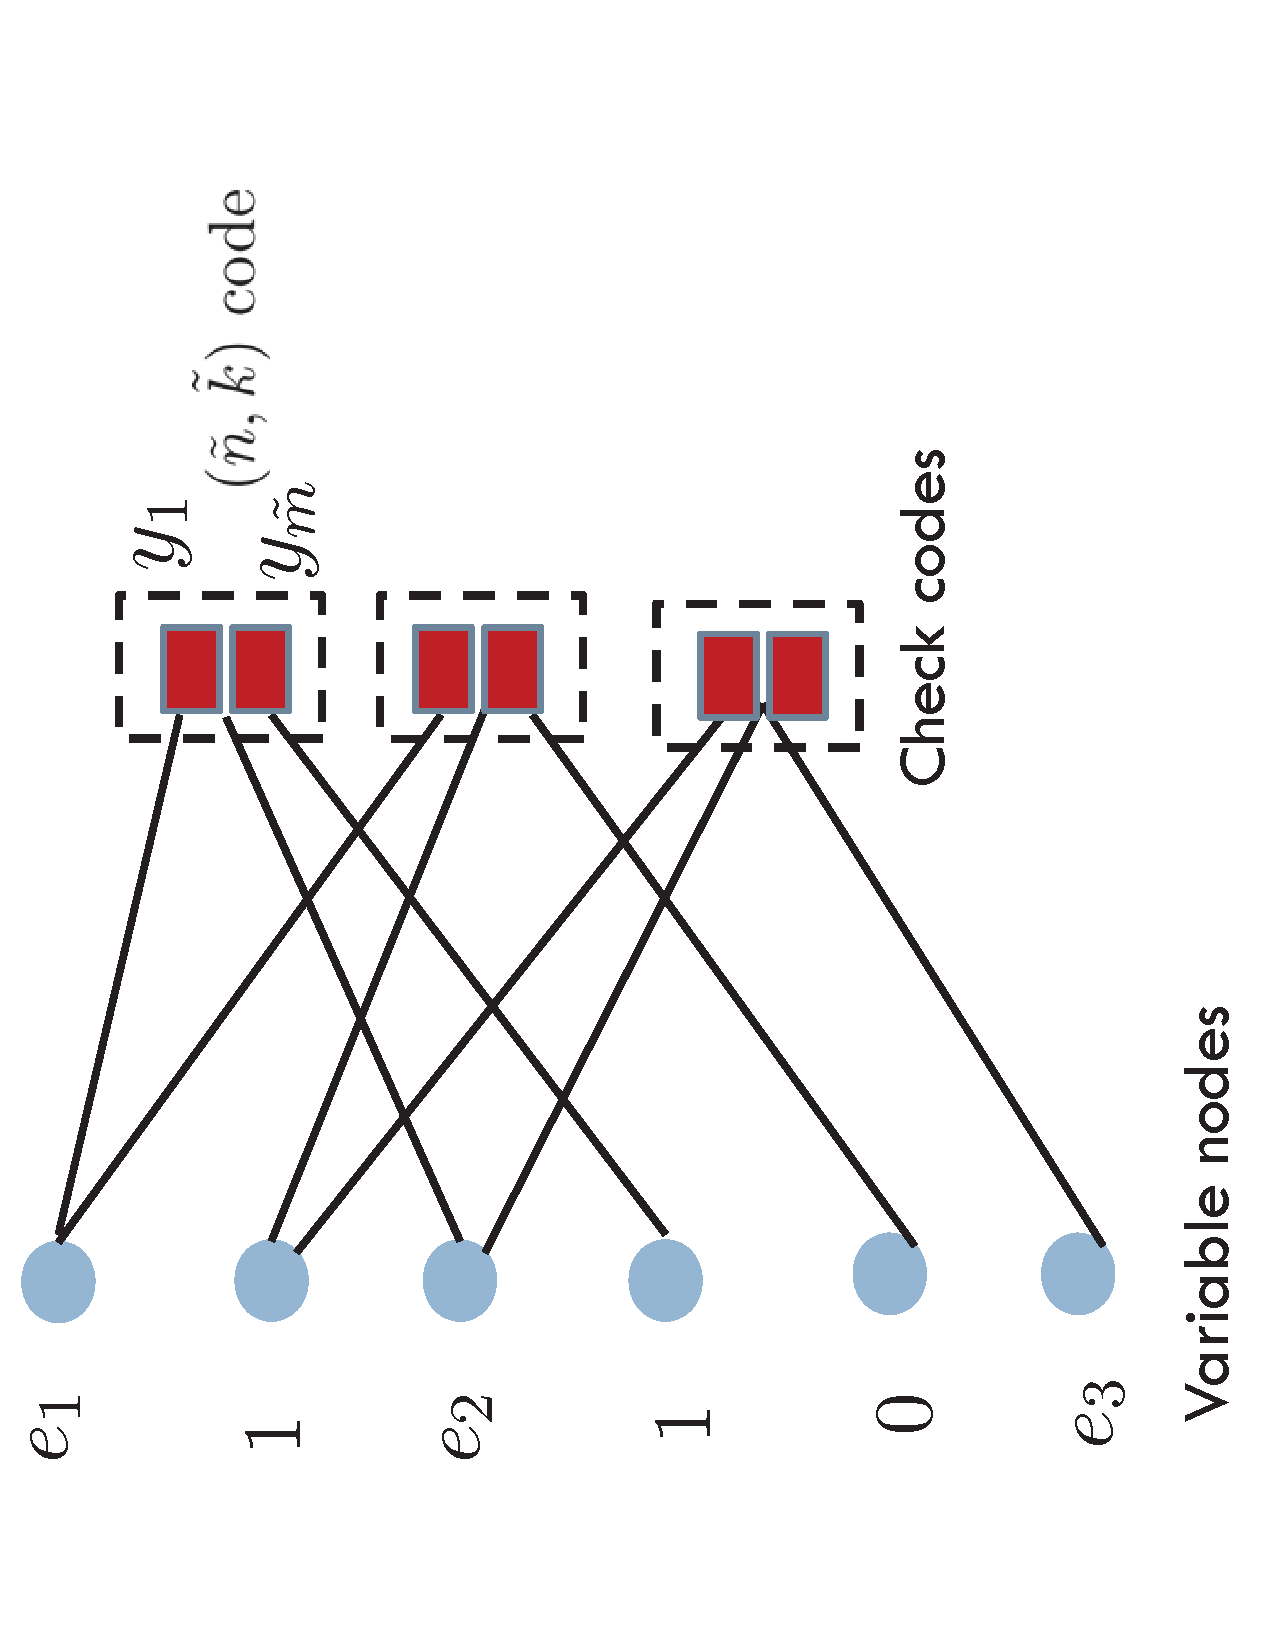
\includegraphics[width=2.0in,angle=-90]{./Figures/GLDPC}
    \end{figure}
\end{columns}
\begin{block}{}
\begin{itemize}
\item $W$ is a primitive element in the field
\item Each check is a 1-error correcting code
\item If there is exactly one error in a check, it can be recovered
\end{itemize}
\end{block}
\end{frame}
%%--------------------------------------------------------------------------------------
%\begin{frame}{Generalized LDPC Code}
%
%\begin{columns}
%    \column{.6\textwidth}
%    .
%%    \small
%%    \[
%%    H = \left[
%%    \begin{array}{ccccccc}
%%    1&0&1&1&0&0\\
%%    1&1&0&0&1&0 \\
%%    0&1&1&0&0&1
%%    \end{array}
%%    \right]
%%    \]
%%    \[
%%    \otimes
%%    \]
%%    \[
%%    T = \left[
%%    \begin{array}{ccccccc}
%%    1&1&1&1&1&1\\
%%    1&W&W^2&W^3&W^4&W^5 \\
%%    \vdots & \vdots & \vdots & \vdots & \vdots & \vdots \\
%%    1&W^{2t-1}&W^{2(2t-1)}&\cdots&\cdots&W^{5(2t-1)}
%%    \end{array}
%%    \right]
%%    \]
%%    \[
%%    \mathbf{\tilde{H}} = H \otimes T
%%    \]
%    \column{.4\textwidth}
%    \begin{figure}[t]
%    \centering
%    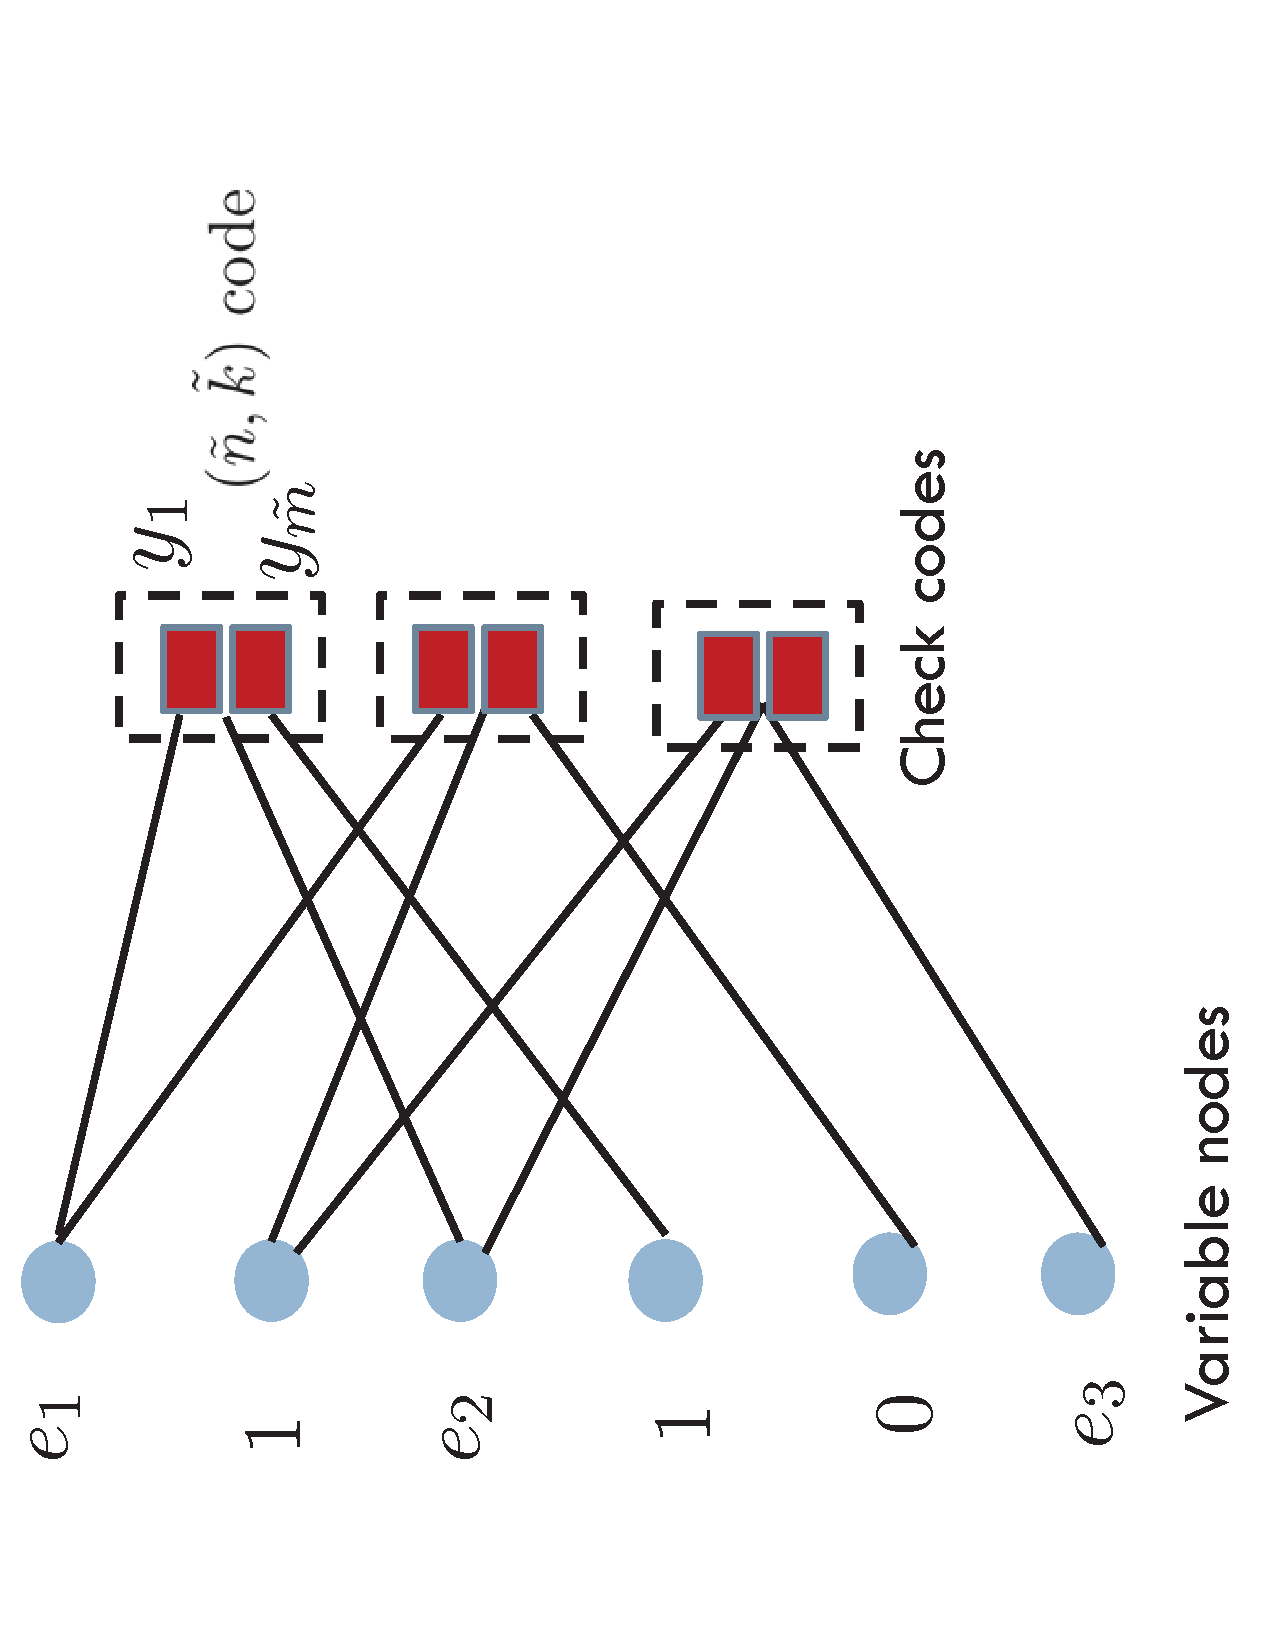
\includegraphics[width=2.0in,angle=-90]{./Figures/GLDPC}
%    \end{figure}
%\end{columns}
%
%\begin{itemize}
%\item GLDPC introduced by Tanner in 1981
%\item Each check is a $t$-error correcting code
%\item If there are exactly $t$ errors in a check, it can be recovered
%\item Density evolution equations can be written and thresholds computed
%\end{itemize}
%
%\end{frame}

%--------------------------------------------------------------------------------------
\begin{frame}{Product code}
\begin{itemize}
\item Special case of generalized LDPC code
\item Let component code $\mathcal{C}$ be an $(\tilde{n},\tilde{k},\tilde{d}_{\text{min}})$ linear code
\item Well-known that \textcolor{blue}{$\mathcal{P}$ is an $(\tilde{n}^{2},\tilde{k}^{2},\tilde{d}_{\text{min}}^{2})$
linear code }
\end{itemize}

\begin{center}
\scalebox{0.8}{\tikzset
{
    vnodeStyle/.style =
    {
        % -- shape properties --
        circle,                                 % shape
        minimum size    = 7mm,                %
        scale           = 1.0,                  % scaling factor
        thick,                                  % thickness of the border
        %
        % -- colours properties --
        % filling: [ trasparent | monocolored | shaded]; decomment what you prefer
%       %                                       % transparent (all commented)
        fill            = yellow!10,             % monocolored
        text            = black,                % colour of the fonts
        draw            = black,                % colour of the border
        %
        % -- fonts --
        font            = \scriptsize,              % shape of the font (or dimension, like \tiny)
%       text centered,                          % text alignment [text centered | text badly centered | text justified | text ragged | text badly ragged]
        inner xsep      = 0mm,                  % minimum distance between text and borders along x dimension
        inner ysep      = 0mm,                  % minimum distance between text and borders along y dimension
        text height     = 0.2cm,
        text depth      = 0.12cm,
    }
}

%\begin{center}
\tikzstyle{styB}=[circle,
  ball color=blue,
  inner sep=0pt,
  minimum size=10pt]
\tikzstyle{styKB}=[circle,
  ball color=blue!10!white,
  inner sep=0pt,
  minimum size=10pt]
\tikzstyle{styCd}=[rectangle, draw=blue!50,
  top color=blue!40!white, bottom color=blue!10,
  inner sep=0pt,
  minimum size=10pt]
\tikzstyle{styCu}=[rectangle, draw=blue,
  top color=blue, bottom color=blue!40,
  inner sep=0pt,
  minimum size=10pt]

\pgfdeclarelayer{background}
%
\pgfdeclarelayer{foreground}
%
\pgfdeclarelayer{m-f}
%
\pgfdeclarelayer{main}
%
\pgfsetlayers{background,main,m-f,foreground}

\begin{tikzpicture}[scale=2.0]
% \draw[step=5mm,color=gray!40!white, thin] (0,0) grid (12,5);

\colorlet{uecolr}{black} \colorlet{decolr}{black!40}

\def\strt  {-40mm}
\def\shf   {10mm}
\def\ang   {55}
\def\dist  {4mm}
\def\cvd   {18mm}

\def\n     {6}
\def\s     {7}

\begin{scope}[xshift=-7cm, yshift=-1.2cm]

\only<1>
{
%\node (cc) at (12mm,5mm) {Product Code\vphantom{y}};

\foreach \rr in {0,1,...,\n}
 \foreach \cc in {0,1,...,\n}
  \node[vnodeStyle] (p\rr\cc) at (\rr*4mm,-\cc*4mm) {$X_{\cc,\rr}$};

 \node [rectangle,rounded corners=2mm,minimum width=7mm,minimum height=55mm,draw=red,thick] (circ1) at (4mm,-12mm) {};
 \node [rectangle,rounded corners=2mm,minimum width=55mm,minimum height=7mm,draw=red,thick] (circ2) at (12mm,-4mm) {};
}

\only<2>
{
%\node (cc) at (12mm,5mm) {Product Code\vphantom{y}};

\foreach \rr in {0,1,...,\n}
 \foreach \cc in {0,1,...,\n}
  \node[vnodeStyle] (p\rr\cc) at (\rr*4mm,-\cc*4mm) {$X_{\cc,\rr}$};

 \node [rectangle,rounded corners=2mm,minimum width=39mm,minimum height=39mm,draw=black,thick] (circ1) at (8mm,-8mm) {};
 \node [rectangle,rounded corners=2mm,minimum width=14mm,minimum height=55mm,draw=blue,thick] (circ1) at (22mm,-12mm) {};
 \node [rectangle,rounded corners=2mm,minimum width=55mm,minimum height=14mm,draw=red,thick] (circ2) at (12mm,-22mm) {};
}

%\only<2>
%{
%\node (cc) at (12mm,5mm) {Symmetric Subcode};
%
%\foreach \cc in {0,1,...,\n}
%  \foreach \rr in {\cc,...,\n}
%    \node[vnodeStyle] (p\rr\cc) at (\rr*4mm,-\cc*4mm) {$X_{\cc,\rr}$};
%
%\pgfmathtruncatemacro{\nnn}{\n-1}
%\foreach \rr in {0,1,...,\nnn} {
%  \pgfmathtruncatemacro{\rrr}{\rr+1}
%  \foreach \cc in {\rrr,...,\n}
%    \node[vnodeStyle] (p\rr\cc) at (\rr*4mm,-\cc*4mm) {$X_{\color{red}{\rr,\cc}}$};
%}
%
% \node [rectangle,rounded corners=2mm,minimum width=7mm,minimum height=55mm,draw=red,thick] (circ1) at (4mm,-12mm) {};
% \node [rectangle,rounded corners=2mm,minimum width=55mm,minimum height=7mm,draw=red,thick] (circ2) at (12mm,-4mm) {};
%}

%\only<3>
%{
%\node (cc) at (12mm,5mm) {Punctured Symmetric Subcode};
%
%\foreach \cc in {0,1,...,\n}
%  \foreach \rr in {\cc,...,\n}
%    \node[vnodeStyle] (p\rr\cc) at (\rr*4mm,-\cc*4mm) {$X_{\cc,\rr}$};
%
% \node [rectangle,rounded corners=2mm,minimum width=7mm,minimum height=15mm,draw=red,thick] (circ1) at (4mm,-2mm) {};
% \node [rectangle,rounded corners=2mm,minimum width=47mm,minimum height=7mm,draw=red,thick] (circ2) at (14mm,-4mm) {};
%}


%\foreach \rr in {0,1,...,\n}{
% \node [rectangle,rounded corners=1mm,minimum width=4mm,minimum height=\n*4mm+4mm,draw=red,thick] (circ1) at (1*4mm,3*4mm) {};
% \node [rectangle,rounded corners=1mm,minimum width=\n*4mm+4mm,minimum height=4mm,draw=maroon,thick] (circ2) at (3*4mm,1*4mm) {};
% \node (cc) at (12mm,29mm) {column codewords};
% \node [rotate=90](rc) at (-6mm,12mm) {row codewords};
% }
\end{scope}

\end{tikzpicture}
%\end{center}
}
\end{center}
\end{frame}

%--------------------------------------------------------------------------------------
\begin{frame}{\alert{Peeling} decoding of product codes}

\begin{itemize}
\item \textcolor{blue}{Hard-decision ``cascade decoding''} by Abramson in 1968
\item Identical to a \alert{peeling decoder}
\item Example: $t=2$-error-correcting codes, bounded distance decoding
\end{itemize}

\begin{columns}
\column{0.65\textwidth}
\begin{center}
\scalebox{1.2}{\pgfdeclarelayer{background}
\pgfdeclarelayer{foreground}
\pgfdeclarelayer{m-f}
\pgfdeclarelayer{main}

\pgfsetlayers{background,foreground}

\begin{tikzpicture}[scale=1.0]
\clip  (-2mm,-2mm) rectangle (26mm, 26mm); 

\def\n     {6}

\begin{pgfonlayer}{background}
%\draw[gray,step=2mm] (-2mm,-2mm) grid (26mm, 26mm);
\foreach \rr in {0,1,...,\n}
 \foreach \cc in {0,1,...,\n}{
  \node[vnodeStyle] (p\rr\cc) at (\rr*4mm,\cc*4mm) {};
 }
\end{pgfonlayer}

\begin{pgfonlayer}{foreground}
\uncover<2-2>{
 \node[minimum width=10cm] (txt) at (12mm,-8mm) {Received block};
}

\uncover<2-3>{
 \foreach \rr/\cc in {1/0,2/0,2/1,0/5,1/4,0/4,6/3,2/4,6/4,3/2,1/3,4/5,3/6,2/2,6/6,6/1}{
  \node[vnodeStyle,thick,fill=red!50,draw=red!80!black!80] (it1\rr\cc)
  at (\cc*4mm,\rr*4mm) {};
 }
}

\uncover<3-4>{
 \node[minimum width=10cm] (txt) at (12mm,-8mm) {Row decoding};
}

\uncover<3-3>{
 \node [rectangle,rounded corners=1mm,minimum width=\n*4mm+4mm,minimum height=4mm,draw=blue,thick] (circ2) at (3*4mm,4*4mm) {};
 \node [rectangle,rounded corners=1mm,minimum width=\n*4mm+4mm,minimum height=4mm,draw=blue,thick] (circ2) at (3*4mm,3*4mm) {};
 \node [rectangle,rounded corners=1mm,minimum width=\n*4mm+4mm,minimum height=4mm,draw=blue,thick] (circ2) at (3*4mm,0*4mm) {};
}

\uncover<4-6>{
 \foreach \rr/\cc in {1/0,2/0,2/1,1/4,6/3,2/4,6/4,1/3,2/2,6/6,6/1}{
  \node[vnodeStyle,thick,fill=red!50,draw=red!80!black!80] (it1\rr\cc)
  at (\cc*4mm,\rr*4mm) {};
 }
}

\uncover<5-6>{
 \node[minimum width=10cm] (txt) at (12mm,-8mm) {Column decoding};
}

\uncover<6-6>{
 \node [rectangle,rounded corners=1mm,minimum width=4mm,minimum height=\n*4mm+4mm,draw=blue,thick] (circ1) at (0*4mm,3*4mm) {};
 \node [rectangle,rounded corners=1mm,minimum width=4mm,minimum height=\n*4mm+4mm,draw=blue,thick] (circ1) at (1*4mm,3*4mm) {};
 \node [rectangle,rounded corners=1mm,minimum width=4mm,minimum height=\n*4mm+4mm,draw=blue,thick] (circ1) at (2*4mm,3*4mm) {};
 \node [rectangle,rounded corners=1mm,minimum width=4mm,minimum height=\n*4mm+4mm,draw=blue,thick] (circ1) at (3*4mm,3*4mm) {};
 \node [rectangle,rounded corners=1mm,minimum width=4mm,minimum height=\n*4mm+4mm,draw=blue,thick] (circ1) at (5*4mm,3*4mm) {};
 \node [rectangle,rounded corners=1mm,minimum width=4mm,minimum height=\n*4mm+4mm,draw=blue,thick] (circ1) at (6*4mm,3*4mm) {};
}

\uncover<7-7>{
 \foreach \rr/\cc in {1/4,2/4,6/4}{
  \node[vnodeStyle,thick,fill=red!50,draw=red!80!black!80] (it1\rr\cc)
  at (\cc*4mm,\rr*4mm) {};
 }
}

\uncover<8-8>{
 \node[minimum width=10cm] (txt) at (12mm,-8mm) {Decoding successful};
}


\uncover<9-9>{
 \node[minimum width=10cm] (txt) at (12mm,-8mm) {Or trapped in a \textcolor{red}{stopping set}};
 \foreach \rr/\cc in {1/0,3/0,6/0,1/2,3/2,6/2,1/5,3/5,6/5}{
  \node[vnodeStyle,thick,fill=red!50,draw=red!80!black!80] (it1\rr\cc)
  at (\cc*4mm,\rr*4mm) {};
 }
}
\end{pgfonlayer}
\end{tikzpicture}}
\end{center}

\column{0.35\textwidth}
\begin{figure}[t]
\centering
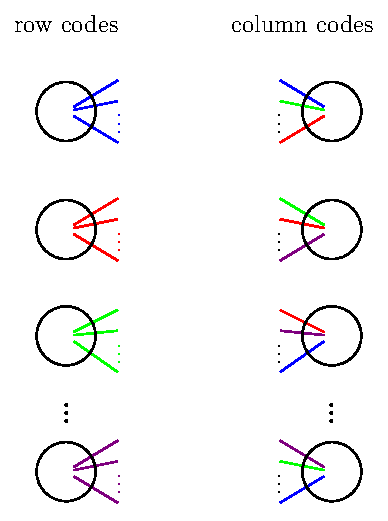
\includegraphics[width=1.3in]{./Figures/Bipartite_graph}
\end{figure}
\end{columns}
\end{frame}

%---------------------------------------------------------------------------------------
\begin{frame}{Density Evolution(DE) for Product Codes -Justesen et al}
%   Slide-1:
%   \begin{itemize}
%   	\item Introduce the main idea of Justesen's analysis (establish the assumptions in the beginning)
%   \end{itemize}
%   Slide-2:
%   \begin{itemize}
%   	\item Tail of the Poisson Distribution. Notion of $\pi_{t}(m)$.
%   	\item Effect- of first step of decoding. Equation for the new mean in therms of $\pi_t(M)$.
%   \end{itemize}

\begin{block}{What is different about DE?}
\begin{itemize}
\item Graph is highly structured
\item Neighborhood is not tree-like
\item Remarkably, randomness in the errors suffices!
\end{itemize}
\end{block}
\pause
   \begin{columns}
   	\column{0.72\textwidth}	   	
   	\begin{block}{Assumptions}
   		\begin{itemize}
   			\item Errors are \alert{randomly distributed} in rows and columns
   			\item \alert{\# errors} in each row/col $\sim$ \alert{Poisson}($M$))
   		\end{itemize}
   	\end{block}
   	\pause
   	\begin{block}{Main Idea}
   		\begin{itemize}
   			%\item Random \alert{bipartite graph} - row and column codes
   			\item Removal of \alert{corrected vertices} (degree$\leq t$) from row codes $\Leftrightarrow$ removal of random edges from column codes uniformly at random
   			\item \# of errors in row/column changes after each iter
   				\item Track the distribution
   				%\item Changes the Poisson parameter ($m(j)$)
   				%\item \alert{Threshold} - max. $M$ such that $m(j) \rightarrow 0$ as $j \rightarrow \infty$
   			%\item Generalize for $d \geq 2$
   		\end{itemize}
   	\end{block}
   	\column{0.25\textwidth}
   	 	
   	\begin{figure}[t]
   		\centering
   		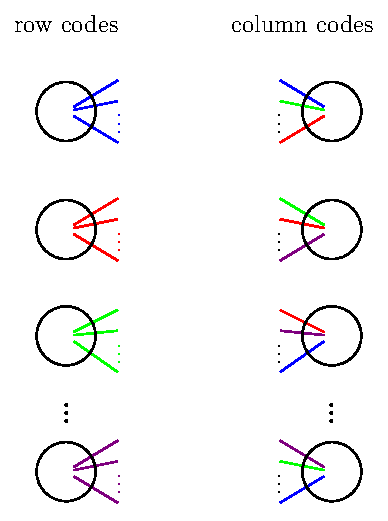
\includegraphics[width=1.3in]{./Figures/Bipartite_graph}
   	\end{figure}
   		
   \end{columns}

\end{frame}
%--------------------------------------------------------------------------------------
\begin{frame}{DE continued}
	\begin{block}{Tail of the Poisson distribution}
		\begin{equation}\nonumber
		\pi_t(m) = \sum_{j \geq t} \mathrm{e}^{-m}m^j/j!
		\label{eqn:defpi}
		\end{equation}
	\end{block}
	
	\begin{block}{Effect of first step of decoding}
		If the \# errors is Poisson with mean $M$, Mean \# of errors after decoding is
		\begin{equation}\nonumber
		\textcolor{blue}{m(1)} = \sum_{j \geq t+1} j\mathrm{e}^{-M}M^j/j! = M\pi_t(M)
		\label{eqn:defpi}
		\end{equation}
	\end{block}
	
\end{frame}
%----------------------------------------------------------------------------------------
\begin{frame}{Evolution of degree distribution($d=2$) - first iteration}
\vspace*{-6mm}
\begin{columns}

\column{0.6\textwidth}
\begin{block}{Row decoding}
\begin{itemize}
\item Before row decoding
    \begin{itemize}
      \item {\color{blue}Distribution}: Poisson($M$), {\color{blue}Mean}: $M$
    \end{itemize}

\item After row decoding
    \begin{itemize}
      \item {\color{blue}Distribution}: Truncated Poisson($M$)
      \item {\color{blue}Mean}: $M \pi_t(M) = m(1)$
    \end{itemize}
\end{itemize}	
\end{block}

\begin{block}{Column decoding}
\begin{itemize}
\item Before column decoding
    \begin{itemize}
      \item {\color{blue}Distribution}: Poisson($m(1)$),{\color{blue}Mean}: $m(1)$
    \end{itemize}

\item After column decoding
    \begin{itemize}
      \item {\color{blue}Distribution}: Truncated Poisson($m(1)$)
      \item {\color{blue}Mean}: $m(2) = M \pi_t(m(1))$
    \end{itemize}
\end{itemize}	
\end{block}

\begin{block}{After every decoding}
\begin{itemize}
  \item Distribution is a Truncated Poisson($m(j)$)
  \item $P[\# errors = i] = b \frac{m(j)^i}{i!}$
\end{itemize}
\end{block}

\column{0.4\textwidth}
\begin{center}
	\vspace{-3mm}
	% This file was created by matlab2tikz.
%
%The latest updates can be retrieved from
%  http://www.mathworks.com/matlabcentral/fileexchange/22022-matlab2tikz-matlab2tikz
%where you can also make suggestions and rate matlab2tikz.
%
\definecolor{mycolor1}{rgb}{0.00000,0.44700,0.74100}%
%
\begin{tikzpicture}

\begin{axis}[%
width=1.521in,
height=0.566in,
at={(0.758in,0.481in)},
scale only axis,
xmin=0,
xmax=15,
ymin=0,
ymax=0.25,
axis background/.style={fill=white}
]
\addplot[ycomb,color=mycolor1,solid,mark=o,mark options={solid},forget plot] plot table[row sep=crcr] {%
0	0.0497870683678639\\
1	0.149361205103592\\
2	0.224041807655388\\
3	0.224041807655388\\
4	0.168031355741541\\
5	0.100818813444924\\
6	0.0504094067224623\\
7	0.0216040314524838\\
8	0.00810151179468143\\
9	0.00270050393156048\\
10	0.000810151179468142\\
11	0.00022095032167313\\
12	5.52375804182826e-05\\
13	1.27471339426806e-05\\
14	2.73152870200298e-06\\
15	5.46305740400597e-07\\
};
\end{axis}
\end{tikzpicture}%
	% This file was created by matlab2tikz.
%
%The latest updates can be retrieved from
%  http://www.mathworks.com/matlabcentral/fileexchange/22022-matlab2tikz-matlab2tikz
%where you can also make suggestions and rate matlab2tikz.
%
\definecolor{mycolor1}{rgb}{0.00000,0.44700,0.74100}%
%
\begin{tikzpicture}

\begin{axis}[%
width=1.521in,
height=0.566in,
at={(0.758in,0.481in)},
scale only axis,
xmin=0,
xmax=15,
ymin=0,
ymax=0.3,
axis background/.style={fill=white}
]
\addplot[ycomb,color=mycolor1,solid,mark=o,mark options={solid},forget plot] plot table[row sep=crcr] {%
0	0\\
1	0\\
2	0.279754460090289\\
3	0.279754460090289\\
4	0.209815845067717\\
5	0.12588950704063\\
6	0.0629447535203151\\
7	0.0269763229372779\\
8	0.0101161211014792\\
9	0.00337204036715975\\
10	0.00101161211014792\\
11	0.000275894211858524\\
12	6.89735529646311e-05\\
13	1.59169737610687e-05\\
14	3.41078009165758e-06\\
15	6.82156018331516e-07\\
};
\end{axis}
\end{tikzpicture}%
	% This file was created by matlab2tikz.
%
%The latest updates can be retrieved from
%  http://www.mathworks.com/matlabcentral/fileexchange/22022-matlab2tikz-matlab2tikz
%where you can also make suggestions and rate matlab2tikz.
%
\definecolor{mycolor1}{rgb}{0.00000,0.44700,0.74100}%
%
\begin{tikzpicture}

\begin{axis}[%
width=1.521in,
height=0.566in,
at={(0.758in,0.481in)},
scale only axis,
xmin=0,
xmax=15,
ymin=0,
ymax=0.4,
axis background/.style={fill=white}
]
\addplot[ycomb,color=mycolor1,solid,mark=o,mark options={solid},forget plot] plot table[row sep=crcr] {%
0	0.347043782149382\\
1	0.367277938616125\\
2	0.194345917046349\\
3	0.0685590420793257\\
4	0.0181390828359174\\
5	0.00383933399474955\\
6	0.000677197300830985\\
7	0.000102382976886822\\
8	1.35440435164562e-05\\
9	1.59263554985051e-06\\
10	1.68549310433711e-07\\
11	1.62160423332975e-08\\
12	1.43012565633619e-09\\
13	1.16423706136106e-10\\
14	8.80083662455855e-12\\
15	6.20930902636336e-13\\
};
\end{axis}
\end{tikzpicture}%
	% This file was created by matlab2tikz.
%
%The latest updates can be retrieved from
%  http://www.mathworks.com/matlabcentral/fileexchange/22022-matlab2tikz-matlab2tikz
%where you can also make suggestions and rate matlab2tikz.
%
\definecolor{mycolor1}{rgb}{0.00000,0.44700,0.74100}%
%
\begin{tikzpicture}

\begin{axis}[%
width=1.521in,
height=0.566in,
at={(0.758in,0.481in)},
scale only axis,
xmin=0,
xmax=15,
ymin=0,
ymax=0.7,
axis background/.style={fill=white}
]
\addplot[ycomb,color=mycolor1,solid,mark=o,mark options={solid},forget plot] plot table[row sep=crcr] {%
0	0\\
1	0\\
2	0.680296442442702\\
3	0.23998689106868\\
4	0.0634947917094919\\
5	0.0134393626461139\\
6	0.00237048928832011\\
7	0.000358385583815417\\
8	4.74101270588406e-05\\
9	5.57492699171389e-06\\
10	5.89996939513159e-07\\
11	5.67633016299058e-08\\
12	5.0060706756166e-09\\
13	4.07534330044602e-10\\
14	3.08068105427641e-11\\
15	2.17353207356291e-12\\
};
\end{axis}
\end{tikzpicture}%
\end{center}

\end{columns}

\end{frame}
%------------------------------------------------------------------------------------------
\begin{frame}{Evolution of the degree distribution - $j$th iteration}


\begin{block}{Recursion}
\begin{itemize}
\item $m(0) = M$
\item $m(1) = M \pi_t(M)$
\item $m(j) = M \pi_t(m(j-1))$
\end{itemize}
\end{block}

\begin{block}{Reduction in the parameter}
\begin{itemize}
  \item Average no. of errors in each row (column) = $m(j) \pi_t(m(j))$
  \item Decoding of rows reduces the parameter by $\frac{m(j) \pi_t(m(j))}{m(j-1) \pi_t(m(j-1))} = \frac{M \pi(m(j))}{m(j-1)}$
  \item New parameter is $m(j+1) = M \pi(m(j))$
\end{itemize}
\end{block}

\begin{block}{Threshold}
In the limit of large $\tilde{n}$ (length in each dimension), a $t$-error correcting product code can correct $\tilde{n}M$ errors when
\[
M < \min_m \displaystyle{\{ \frac{m}{\pi_t(m)} \}}
\]
\end{block}

\end{frame}
%------------------------------------------------------------------------------------------
%\begin{frame}{Evolution of degree distribution - $j$th iteration}
%\begin{columns}
%
%\column{0.55\textwidth}
%{\vspace{-6mm}
%	\hspace{6mm}
%	\begin{block}{Before row decoding}
%		{\color{blue}Distribution}: Poisson($m(j)$) \\
%	\end{block}}
%	\vspace{6mm}
%	\begin{block}{After row decoding}
%		{\color{blue}Distribution}: Truncated Poisson($m(j)$) \\
%		{\color{blue}Mean}: $m(j) \pi_t(m(j))$ \\
%		{\color{blue}Reduction by a factor}: $\frac{m(j) \pi_t(m(j))}{m(j-1) \pi_t(m(j-1))}$ \\
%	\end{block}
%	\column{0.45\textwidth}
%	\begin{center}
%		\vspace{-3mm}
%		% This file was created by matlab2tikz.
%
%The latest updates can be retrieved from
%  http://www.mathworks.com/matlabcentral/fileexchange/22022-matlab2tikz-matlab2tikz
%where you can also make suggestions and rate matlab2tikz.
%
\definecolor{mycolor1}{rgb}{0.00000,0.44700,0.74100}%
%
\begin{tikzpicture}

\begin{axis}[%
width=1.521in,
height=0.566in,
at={(0.758in,0.481in)},
scale only axis,
xmin=0,
xmax=15,
ymin=0,
ymax=0.25,
axis background/.style={fill=white}
]
\addplot[ycomb,color=mycolor1,solid,mark=o,mark options={solid},forget plot] plot table[row sep=crcr] {%
0	0.0497870683678639\\
1	0.149361205103592\\
2	0.224041807655388\\
3	0.224041807655388\\
4	0.168031355741541\\
5	0.100818813444924\\
6	0.0504094067224623\\
7	0.0216040314524838\\
8	0.00810151179468143\\
9	0.00270050393156048\\
10	0.000810151179468142\\
11	0.00022095032167313\\
12	5.52375804182826e-05\\
13	1.27471339426806e-05\\
14	2.73152870200298e-06\\
15	5.46305740400597e-07\\
};
\end{axis}
\end{tikzpicture}%
%		% This file was created by matlab2tikz.
%
%The latest updates can be retrieved from
%  http://www.mathworks.com/matlabcentral/fileexchange/22022-matlab2tikz-matlab2tikz
%where you can also make suggestions and rate matlab2tikz.
%
\definecolor{mycolor1}{rgb}{0.00000,0.44700,0.74100}%
%
\begin{tikzpicture}

\begin{axis}[%
width=1.521in,
height=0.566in,
at={(0.758in,0.481in)},
scale only axis,
xmin=0,
xmax=15,
ymin=0,
ymax=0.3,
axis background/.style={fill=white}
]
\addplot[ycomb,color=mycolor1,solid,mark=o,mark options={solid},forget plot] plot table[row sep=crcr] {%
0	0\\
1	0\\
2	0.279754460090289\\
3	0.279754460090289\\
4	0.209815845067717\\
5	0.12588950704063\\
6	0.0629447535203151\\
7	0.0269763229372779\\
8	0.0101161211014792\\
9	0.00337204036715975\\
10	0.00101161211014792\\
11	0.000275894211858524\\
12	6.89735529646311e-05\\
13	1.59169737610687e-05\\
14	3.41078009165758e-06\\
15	6.82156018331516e-07\\
};
\end{axis}
\end{tikzpicture}%
%	\end{center}
%\end{columns}
%
%
%\begin{block}{d-stages}
%	
%	\begin{center}
%		\begin{itemize}
%			\item  $m(j)= M \ \prod \limits_{i=1}^{d-1}{\pi_t(m(j-i))}$
%			\item $\frac{m(j)}{m(j-d)}=\frac{M\prod\limits_{i=1}^{d-1} \pi_t(m(j-i))}{m(j-d)} \leq M \frac{\pi_t^{d-1}(m(j-d))}{m(j-d)}$
%		\end{itemize}
%	\end{center}
%	
%\end{block}
%\end{frame}

%----------------------------------------------------------------------------------------
	\begin{frame}{Thresholds for asymptotically large field size}
	%	\begin{itemize}
	%		
	%	\item Theorem for the Threshold value for Less-sparse case.
	%	\item Table showing threshold values for different $d$ and $t$.
	%	\item Highlight some useful points in the table {\bf(if needed)}
	%	\end{itemize}
		
		\begin{block}{}
			\begin{center}
				\alert{Threshold} = $ \frac{\# \ of parity symbols}{\# \ of errors}$
			\end{center}
			
			\vspace{-6mm}
			\color{black}
			\begin{table}[ht]
				\centering
				\begin{tabular}{c|ccccccc}
					\hline
					& $d=2$ & $d=3$ & $d=4$ & $d=5$ & $d=6$ & $d=7$ & $d=8$ \\
					\hline
					\rowcolor{lightgray}
					$t=1$& 4.0  & 2.4436 & 2.5897 & 2.8499 & 3.1393 & 3.4378 & 3.7383 \\
					$t=2$& 2.3874 & 2.5759 & 2.9993 & 3.4549 & 3.9153 & 4.3736 & 4.8278 \\
					\rowcolor{lightgray}
					$t=3$& 2.3304 & 2.7593 & 3.3133 & 3.8817 & 4.4483 & 5.0094 & 5.5641 \\
					$t=4$& 2.3532 & 2.9125 & 3.5556& 4.2043 & 4.8468 & 5.4802 & 6.1033 \\
					%\rowcolor{lightgray}
					%$t=5$& 2.3908 & 3.0394 & 3.7471 & 4.4500 & 5.1362 & 5.8018 & 6.4451 \\
					
					\hline
				\end{tabular}
			\end{table}
			\vspace{-3mm}
			
			Notice that $L,K = O \left( N^{\frac{1-d}{d}}\right)$
		\end{block}
	\end{frame}
%--------------------------------------------------------------------------------------
\begin{frame}{Syndrome source coding}

\begin{columns}
\column{0.5\textwidth}
\begin{center}
  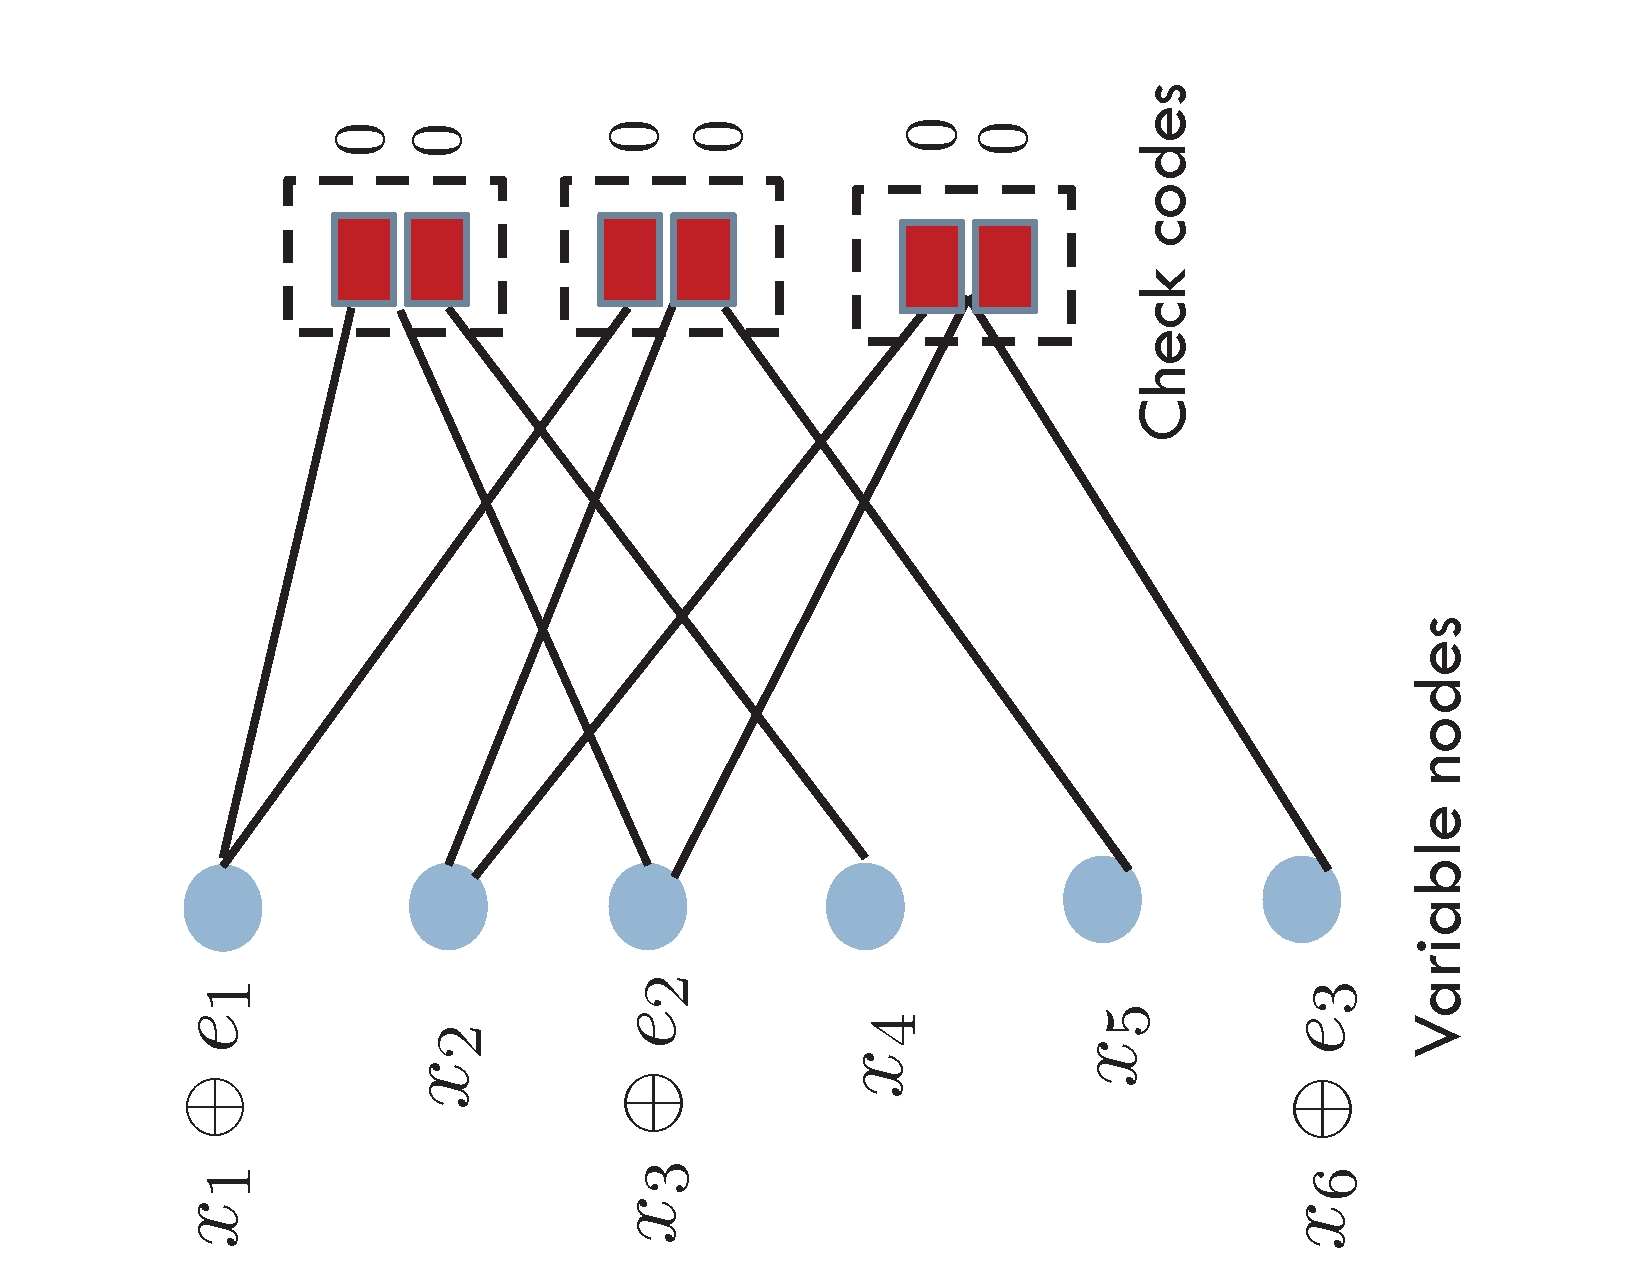
\includegraphics[width=2.0in,angle=-90]{./Figures/syndromesourcecoding2_1}
\end{center}
\begin{itemize}
  \item $H \underline{x} = 0$
  \item Receive - $\underline{r} = \underline{x} \oplus \underline{e}$
  \item $H \underline{r} = H \underline{e} = \underline{y}$
  \item Recover $\xv$ and sparse $\ev$
\end{itemize}
\column{0.5\textwidth}
\begin{center}
  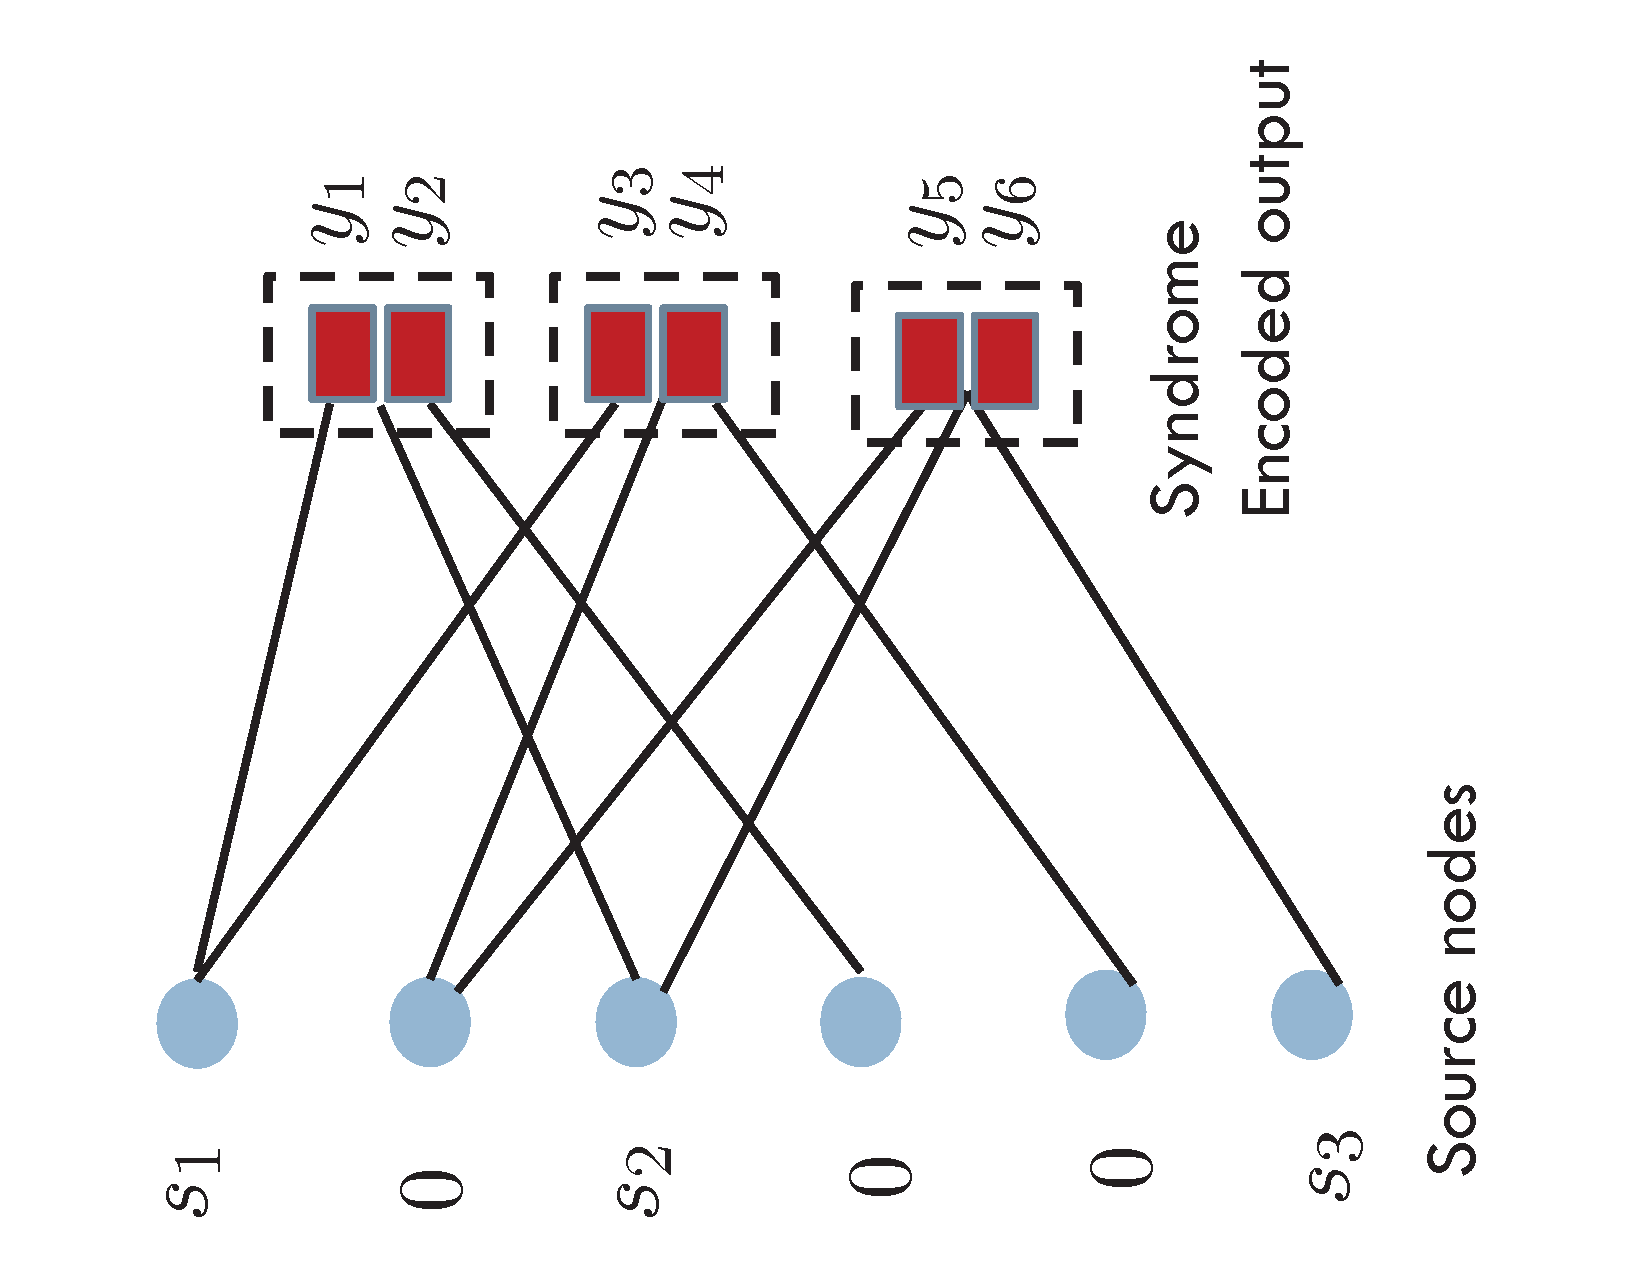
\includegraphics[width=2.0in,angle=-90]{./Figures/syndromesourcecoding2_2}
\end{center}
\begin{itemize}
  \item $H \underline{s} = \underline{y}$
  \item Set $\underline{r} = 0 $ (Let a genie add $\underline{x}$ to $\underline{r}$)
  \item $\underline{y}$ is given to the decoder
  \item Recover sparse $\sv$
\end{itemize}
\end{columns}
\end{frame}
